\documentclass[12pt]{article}

% packages :
\usepackage[utf8x]{inputenc}
\usepackage[T1]{fontenc}
%\usepackage[francais]{babel}
%
\usepackage{graphicx} % images
\usepackage{float}
\usepackage{placeins}
\usepackage{multirow}
\usepackage{wrapfig}
\usepackage{array}

% to draw circuits
\usepackage{siunitx}
\usepackage[siunitx]{circuitikz}
\usetikzlibrary{calc}

\usepackage[top=2cm, bottom=2cm, left=2.5cm, right=2.5cm]{geometry}


% maths :
\usepackage{amsthm}
\usepackage{amsmath}
\usepackage{amssymb}
\usepackage{mathrsfs}

\begin{document}

% ENSEMBLE DES CIRCUITS PRÉSENTS DANS LE TUTORIEL

\begin{center}
\begin{circuitikz}
\draw (0,0) to[battery] (0,3) to[closing switch, l=$a$] (3,3)  to[lamp,l=$a$] (3,0) -- (0,0);
\end{circuitikz}
\end{center}

\begin{center}
\begin{circuitikz}
\draw (0,0) to[battery] (0,3) to[open]  (3,3)  to[lamp,l=$\bar{a}$] (3,0) -- (0,0);
\draw (1,3) node[spdt] (s) {};
\draw (s.in) node[anchor=south west]{$a$};
\draw (s.out 1) node[above]{\small 0} -- (3,3.315) -- (3,3);
\draw (s.out 2) node[below]{\small 1} -- +(.41,0) -- (2,0.5) to[R,-*] (0,.5);
\draw (0,3) -- (s.in);
\end{circuitikz}
\end{center}

\begin{center}
\begin{circuitikz}
\draw (0,0) to[battery] (0,3) -- (1,3) to[short,*-] (1,3.5) to[closing switch, l=$a$] (2,3.5) to[short,-*] (2,3) -- (3,3)  to[lamp,l=$a+b$] (3,0) -- (0,0);
\draw (1,3) -- (1,2.5) to[closing switch, l=$b$] (2,2.5) -- (2,3);
\end{circuitikz}
\end{center}

\begin{center}
\begin{circuitikz}
\draw (0,0) to[battery] (0,3) to[closing switch, l=$a$] (1.5,3) to[closing switch, l=$b$] (3,3) to[lamp,l=$a\cdot b$] (3,0) -- (0,0);
\end{circuitikz}
\end{center}

\begin{center}
\begin{circuitikz}
\draw (0,0) to[Do,*-*] (2,0);
\end{circuitikz}
\end{center}


\begin{center}
\begin{circuitikz}
\draw (2,-3) node[ground] (g) {};
\draw (0,0) node[left]{$a$} to[Do,*-] (2,0) to [short, -*] (2,-1);
\draw (0,-1) node[left]{$b$} to[Do,*-] +(2,0) to[short,-*] +(1,0) node[right]{$a+b$};
\draw (2,-1) to[R=$R_L$] (g);
\end{circuitikz}
\end{center}

\begin{center}
\begin{circuitikz}
\draw (2,-1) to[short,*-] (2,0) to[Do,-*] (0,0) node[left]{$a$};
\draw (3,-1) node[right]{$a\cdot b$}  to[short,*-] +(-1,0) to[Do,-*] +(-2,0) node[left]{$b$};
\draw (2,0) to[R=$R_L$,*-*] +(0,2) node[above]{$+V$};
\end{circuitikz}
\end{center}

\begin{center}
\begin{circuitikz}
\draw (0,0) node[npn] (x) {};
\draw (x.B) node[left]{B};
\draw (x.C) node[above]{C};
\draw (x.E) node[below]{E};

\draw (3,0) node[pnp] (y) {};
\draw (y.B) node[left]{B};
\draw (y.C) node[below]{C};
\draw (y.E) node[above]{E};
\end{circuitikz}
\end{center}


\begin{center}
\begin{circuitikz}
\draw (0,0) node[npn] (x) {};
\draw (0,-1) node[ground] (g) {};
\draw (x.B) to[R,-*] +(-1.5,0) node[left]{$a$};
\draw (x.C) to[R,-*] +(0,1.5) node[above]{$+V$};
\draw (x.C) to[short,*-*] +(1,0) node[right]{$\bar{a}$};
\draw (x.E) to[short] (g);
\end{circuitikz}
\end{center}

\begin{center}
\begin{circuitikz}
\draw (0,0) node[npn] (x) {};
\draw (0,-2) node[npn] (y) {};
\draw (x.E) to[short] (y.C);
\draw (0,-4.75) node[ground] (g) {};
\draw (x.B) to[R,-*] +(-1.5,0) node[left]{$a$};
\draw (y.B) to[R,-*] +(-1.5,0) node[left]{$b$};
\draw (x.C) to[short,-*] +(0,.25) node[above]{$+V$};
\draw (y.E) to[short,*-*] +(1,0) node[right]{$a\cdot b$};
\draw (y.E) to [short] +(0,-.5) to[R] (g);
\end{circuitikz}
\end{center}

\begin{center}
\begin{circuitikz}
\draw (0,0) node[npn] (x) {};
\draw (0,-2) node[npn] (y) {};
% \draw (x.E) to[short] (y.C);
\draw (0,-4.75) node[ground] (g) {};
\draw (x.B) to[R,-*] +(-1.5,0) node[left]{$a$};
\draw (y.B) to[R,-*] +(-1.5,0) node[left]{$b$};
\draw (x.C) to[short] +(1,0) to[short,-*] +(0,. 5) node[above]{$+V$};
\draw (y.E) to[short,*-*] +(2,0) node[right]{$a+ b$};
\draw(x.E) to[short] +(.75,0) to [short,-*] +(0,-2);
\draw (y.C) to[short] +(1,0) to [short,-*] +(0,2);
\draw (y.E) to [short] +(0,-.5) to[R] (g);
\end{circuitikz}
\end{center}

\begin{center}
\begin{circuitikz}
\draw (0,0) node[nmos] (x) {};
\draw (x.G) node[left]{G};
\draw (x.D) node[above]{D};
\draw (x.S) node[below]{S};

\draw (3,0) node[pmos] (y) {};
\draw (y.B) node[left]{G};
\draw (y.D) node[below]{D};
\draw (y.S) node[above]{S};
\end{circuitikz}
\end{center}

\begin{center}
\begin{circuitikz}
\draw (0,0) node[pmos] (x) {};
\draw (0,-1.5) node[nmos] (y) {};
\draw (0,-2.25) node[ground] (g) {};
\draw (x.D) to[short] (y.C);
\draw (x.S) to[short,-*] +(0,.25) node[above]{$+V$};
\draw (y.E) to[short] (g);
\draw (x.D) to [short,*-*] ++(1,0) node[right]{$\bar{a}$};
\draw (x.G) to[short] (y.G);
\draw (x.G) ++(0,-.75) to[short,*-*] ++(-1,0) node[left]{$a$};
\end{circuitikz}
\end{center}

\begin{center}
\begin{circuitikz}
\draw (0,0) node[pmos] (x) {};
\draw (0,-1.5) node[nmos] (y) {};
\draw (0,-2.25) node[ground] (g) {};
\draw (x.D) to[short] (y.C);
\draw (x.S) to[short,-*] +(0,.25) node[above]{$+V$};
\draw (y.E) to[short] (g);
\draw (x.D) to [short,*-*] ++(1,0) node[right]{$\overline{(a+b)}$};
%\draw (x.G) to[short] (y.G); 
\draw (x.G) to[short,-*] +(-.5,0) node [left]{$a$};
\draw (y.G) to[short,-*] +(-.5,0) node [left]{$b$};
%\draw (x.G) ++(0,-.75) to[short,*-*] ++(-1,0) node[left]{$a$};
\end{circuitikz}
\end{center}

\begin{center}
\begin{circuitikz}
\draw (-1,1.75) node[pmos] (p1) {};
\draw (1,1.75) node[pmos] (p2) {};
\draw (0,0) node[nmos] (n1) {};
\draw (0,-1.5) node[nmos] (n2) {};
\draw (0,-2.25) node[ground] (g) {};
\draw (n1.S) to[short] (n2.D);

\draw (p1.S) to[short] (p2.S);
\draw (p1.D) to[short] (p2.D);
\draw (n1.D) to[short,-*] +(0,.2);

\draw (0,2.52) to[short,*-*] +(0,.5) node[above]{$+V$}; 
\draw (n1.G) to[short] +(-1,0) to[short] (p1.G); 
\draw (n2.G) to[short] ++(-.25,0) to[short] ++(0,2) to[short] ++(.5,0) to[short] ++(0,1.25) to[short] (p2.G);

\draw (n1.D) ++(0,-.25) to[short,*-*] +(1,0) node[right]{$\overline{a\cdot b}$};
\draw (n2.G)  ++(-.25,0) ++(0,1) to[short, *-*] ++(-1,0) node[left]{$b$};
\draw (n1.G) ++(-1,0) ++(0,.5) to[short, *-*] ++(-1,0) node[left]{$a$};
\end{circuitikz}
\end{center}

\begin{center}
\begin{circuitikz}
\draw (0,0) node[not port] (notx) {};
\draw (notx.in) to[short,-*] +(-.5,0) node[left] {$a$};
\draw (notx.out) to[short,-*] +(.5,0) node[right] {$\bar{a}$};
\end{circuitikz}
\end{center}

\begin{center}
\begin{circuitikz}
\draw (0,0) node[and port] (andx) {};
\draw (andx.in 1) to[short,-*] +(-.5,0) node[left] {$a$};
\draw (andx.in 2) to[short,-*] +(-.5,0) node[left] {$b$};
\draw (andx.out) to[short,-*] +(.5,0) node[right] {$a\cdot b$};
\end{circuitikz}
\end{center}

\begin{center}
\begin{circuitikz}
\draw (0,0) node[or port] (orx) {};
\draw (orx.in 1) to[short,-*] +(-.5,0) node[left] {$a$};
\draw (orx.in 2) to[short,-*] +(-.5,0) node[left] {$b$};
\draw (orx.out) to[short,-*] +(.5,0) node[right] {$a+b$};
\end{circuitikz}
\end{center}

\begin{center}
\begin{circuitikz}
\draw (0,0) node[nand port] (andx) {};
\draw (andx.in 1) to[short,-*] +(-.5,0) node[left] {$a$};
\draw (andx.in 2) to[short,-*] +(-.5,0) node[left] {$b$};
\draw (andx.out) to[short,-*] +(.5,0) node[right] {$a\uparrow b = \overline{a\cdot b}$};
\end{circuitikz}
\end{center}

\begin{center}
\begin{circuitikz}
\draw (0,0) node[nor port] (orx) {};
\draw (orx.in 1) to[short,-*] +(-.5,0) node[left] {$a$};
\draw (orx.in 2) to[short,-*] +(-.5,0) node[left] {$b$};
\draw (orx.out) to[short,-*] +(.5,0) node[right] {$a\downarrow b = \overline{a+b}$};
\end{circuitikz}
\end{center}
\begin{center}

\begin{circuitikz}
\draw (0,0) node[xor port] (orx) {};
\draw (orx.in 1) to[short,-*] +(-.5,0) node[left] {$a$};
\draw (orx.in 2) to[short,-*] +(-.5,0) node[left] {$b$};
\draw (orx.out) to[short,-*] +(.5,0) node[right] {$a\oplus b = (a+b)\overline{(a\cdot b)}$};
\end{circuitikz}
\end{center}


\begin{center}

\begin{circuitikz}
\def\lll{7.5}
\draw (0,-.5) node[left]{$a$} -- +(\lll,0);
\draw (0,-1) node[left]{$b$} -- +(\lll,0);
\draw (1,-2) node[not port] (notb) {};
\draw (.25,-1) to[short,*-] ++(0,-1) -- (notb.in);
\draw (notb.out) node[below,blue]{$\bar{b}$} -- (\lll,-2) ;

\draw (0,-3) node[left]{$c$} -- +(\lll,0);
\draw (1,-4) node[not port] (notc) {};
\draw (.25,-3) to[short,*-] ++(0,-1) -- (notc.in);
\draw (notc.out)node[below,blue]{$\bar{c}$} -- (\lll,-4);

\draw (2.25,-6) node[and port,rotate=-90] (and1) {};
\draw (and1.in 1) to [short, -*] +(0,4.1);
\draw (and1.in 2) to [short, -*] +(0,3.6);
\draw (and1.out) node[blue,left]{$a\cdot b$};


\draw (2.75,-8) node[and port,rotate=-90] (and2) {};
\draw (and2.in 1) to [short, -*] +(0,2.6);
\draw (and2.in 2) to[short] +(0,.45) to[short] (and1.out);
\draw (and2.out) node[blue,left]{$a\cdot b\cdot \bar{c}$};

\draw (4.25,-6) node[and port,rotate=-90] (and3) {};
\draw (and3.in 1) to [short, -*] +(0,4.1);
\draw (and3.in 2) to [short, -*] +(0,2.6);
\draw (and3.out) node[blue,left]{$a\cdot \bar{b}$};


\draw (4.75,-8) node[and port,rotate=-90] (and4) {};
\draw (and4.in 1) to [short, -*] +(0,3.6);
\draw (and4.in 2) to[short] +(0,.45) to[short] (and3.out);
\draw (and4.out) node[blue,left]{$a\cdot \bar{b}\cdot c$};

\draw (6.25,-6) node[and port,rotate=-90] (and5) {};
\draw (and5.in 1) to [short, -*] +(0,4.1);
\draw (and5.in 2) to [short, -*] +(0,2.6);
\draw (and5.out) node[blue,left]{$a\cdot \bar{b}$};


\draw (6.75,-8) node[and port,rotate=-90] (and6) {};
\draw (and6.in 1) to [short, -*] +(0,2.6);
\draw (and6.in 2) to[short] +(0,.45) to[short] (and5.out);
\draw (and6.out) node[blue,left]{$a\cdot \bar{b}\cdot \bar{c}$};

\draw (6.5,-10) node[or port] (or1) {};
\draw (and2.out) -- +(0,-2.125) -- (or1.in 2);
\draw (and4.out) -- +(0,-1.57) -- (or1.in 1);

\draw (and6.out) ++(2,-1) node[or port] (or2) {};
\draw (and6.out)  -- ++(0,-.72) -- (or2.in 1);
\draw (or1.out) node[below=.4cm,blue]{$a\cdot b\cdot \bar{c}+a\cdot \bar{b}\cdot c$} -- ++(0.25,0) -- ++(0,0.565) -- (or2.in 2);
\draw (or2.out) to[short,-*] +(.5,0) node[right]{$a\cdot b\cdot \bar{c}+a\cdot \bar{b}\cdot c+a\cdot \bar{b}\cdot \bar{c}$};
\end{circuitikz}
\end{center}



\begin{center}

\begin{circuitikz}
\def\lll{5}
\draw (0,0) node[left]{$a$} -- +(\lll,0);

\draw (1,-1) node[not port] (notb) {};
\draw (0,-1) node[left]{$b$} -- (notb.in);
\draw (notb.out) node[below,blue]{$\bar{b}$} -- (\lll,-1) ;

\draw (1,-2.5) node[not port] (notc) {};
\draw (0,-2.5) node[left]{$c$} -- (notc.in);
\draw (notc.out)node[below,blue]{$\bar{c}$} -- (\lll,-2.5);

\draw (2.5,-5) node[and port,rotate=-90] (and1) {};
\draw (and1.in 1) to [short, -*] +(0,2.6);
\draw (and1.in 2) to [short, -*] +(0,3.6);
\draw (and1.out) node[blue,left]{$a\cdot \bar{b}$};

\draw (4,-5) node[and port,rotate=-90] (and2) {};
\draw (and2.in 1) to [short, -*] +(0,1.1);
\draw (and2.in 2) to [short, -*] +(0,3.6);
\draw (and2.out) node[blue,left]{$a\cdot \bar{c}$};


\draw (5.5,-6) node[or port] (or1) {};
\draw (and1.out) -- +(0,-1.125) -- (or1.in 2);
\draw (and2.out) -- +(0,-0.57) -- (or1.in 1);

\draw (or1.out) to[short,-*] +(.5,0) node[right]{$a\cdot \bar{b}+a\cdot \bar{c}$};
\end{circuitikz}
\end{center}

\begin{center}

\begin{circuitikz}
\def\lll{4}
\draw (0,0) node[left]{$a$} -- +(\lll,0);

\draw (1,-1) node[not port] (notb) {};
\draw (0,-1) node[left]{$b$} -- (notb.in);
\draw (notb.out) node[below,blue]{$\bar{b}$} -- (\lll,-1) ;

\draw (1,-2.5) node[not port] (notc) {};
\draw (0,-2.5) node[left]{$c$} -- (notc.in);
\draw (notc.out)node[below,blue]{$\bar{c}$} -- (\lll,-2.5);

\draw (2.5,-5) node[or port,rotate=-90] (or1) {};
\draw (or1.in 1) to [short, -*] +(0,1.1);
\draw (or1.in 2) to [short, -*] +(0,2.6);
\draw (or1.out) node[blue,left]{$\bar{b}+ \bar{c}$};


\draw (5,-6) node[and port] (and1) {};
\draw (or1.out) -- +(0,-1.125) -- (and1.in 2);
\draw (and1.in 1) to[short,-*] +(0,5.72);

\draw (and1.out) to[short,-*] +(.5,0) node[right]{$a\,(\bar{b}+\bar{c})$};
\end{circuitikz}
\end{center}

\begin{center}

\begin{circuitikz}

\draw (2,-1) node[nand port] (nand) {};
\draw (nand.in 1) -- +(-.5,0) node[left]{$b$};
\draw (nand.in 2) -- +(-.5,0) node[left]{$c$};

\draw (4,0) node[and port] (and) {};
\draw (nand.out) node[below=.4cm,blue]{$\overline{b\cdot c}$}-- ++ (.47,0) --  (and.in 2);
\draw (and.in 1) -- +(-2.5,0) node[left]{$a$};
\draw (and.out) to[short,-*] +(.5,0) node[right]{$a\,\overline{(b\cdot c)}$};
\end{circuitikz}
\end{center}


\begin{center}
\begin{circuitikz}

\draw (0,.25) -- (0,-1.25) -- (.5,-1) -- (.5,0) -- cycle;
\draw (0,-.2) node[right]{\small 0} -- +(-.5,0) node[left]{$e_0$};
\draw (0,-.8) node[right]{\small 1} -- +(-.5,0) node[left]{$e_1$};
\draw (.5,-.5) to[short,-*] +(.5,0) node[right]{$q$};
\draw (.25,.125) -- +(0,.5) node[above]{$s_0$};
\end{circuitikz}
\end{center}

\begin{center}

\begin{circuitikz}
\def\lll{5}
\draw (0,0) node[left]{$s_0$} -- +(\lll,0);
\draw (1,-1) node[not port] (nots) {};
\draw (.25,0) to[short,*-] ++(0,-1) -- (nots.in);
\draw (nots.out) node[below,blue]{$\overline{s_0}$} -- (\lll,-1) ;

\draw (0,-2) node[left]{$e_0$} -- +(\lll,0);
\draw (0,-3) node[left]{$e_1$} -- +(\lll,0);


\draw (2.5,-5) node[and port,rotate=-90] (and1) {};
\draw (and1.in 1) to [short, -*] +(0,1.6);
\draw (and1.in 2) to [short, -*] +(0,2.6);
\draw (and1.out) node[blue,left]{$\overline{s_0}\cdot e_0$};

\draw (4,-5) node[and port,rotate=-90] (and2) {};
\draw (and2.in 1) to [short, -*] +(0,3.6);
\draw (and2.in 2) to [short, -*] +(0,0.6);
\draw (and2.out) node[blue,left]{$s_0\cdot e_1$};


\draw (6,-6) node[or port] (or1) {};
\draw (and1.out) -- +(0,-1.125) -- (or1.in 2);
\draw (and2.out) -- +(0,-0.56) -- (or1.in 1);

\draw (or1.out) to[short,-*] +(.5,0) node[right]{$\overline{s_0} \cdot e_0 + s_0\cdot e_1$};
\end{circuitikz}
\end{center}


\begin{center}
\begin{circuitikz}

\begin{scope}[xshift=-4cm,yshift=-.75cm]
\draw (0,.25) -- (0,-2.25) -- (1,-2) -- (1,0) -- cycle;
\draw (0,-.2) node[right]{\small 0} -- +(-.5,0) node[left]{$e_0$};
\draw (0,-.75) node[right]{\small 1} -- +(-.5,0) node[left]{$e_1$};
\draw (0,-1.25) node[right]{\small 2} -- +(-.5,0) node[left]{$e_2$};
\draw (0,-1.8) node[right]{\small 3} -- +(-.5,0) node[left]{$e_3$};
\draw (1,-1) -- +(.5,0) node[right]{q};
\draw (.25,.18) -- +(0,.5) node[above]{$s_0$};
\draw (.75,.07) -- +(0,.5) node[above]{$s_1$};
\end{scope}

\begin{scope}
\draw (0,.25) -- (0,-1.25) -- (.5,-1) -- (.5,0) -- cycle;
\draw (0,-.2) node[right]{\small 0} -- +(-.5,0) node[left]{$e_0$};
\draw (0,-.8) node[right]{\small 1} -- +(-.5,0) node[left]{$e_1$};
\draw (.5,-.5) -- +(.5,0);
\draw (.25,.125) -- +(0,.5) node[above]{$s_0$};
\end{scope}

\begin{scope}[yshift=-2cm]
\draw (0,.25) -- (0,-1.25) -- (.5,-1) -- (.5,0) -- cycle;
\draw (0,-.2) node[right]{\small 0} -- +(-.5,0) node[left]{$e_2$};
\draw (0,-.8) node[right]{\small 1} -- +(-.5,0) node[left]{$e_3$};
\draw (.5,-.5) -- +(.5,0);
\draw (.25,-1-.125) -- +(0,-.5) node[below]{$s_0$};
\end{scope}

\begin{scope}[yshift=-1cm,xshift=1.5cm]
\draw (0,.25) -- (0,-1.25) -- (.5,-1) -- (.5,0) -- cycle;
\draw (0,-.2) node[right]{\small 0} -- ++(-.5,0) -- ++(0,.7);
\draw (0,-.8) node[right]{\small 1} -- ++(-.5,0) -- ++(0,-.7);
\draw (.5,-.5) -- +(.5,0) node[right]{$q$};
\draw (.25,.125) -- +(0,.5) node[above]{$s_1$};
\end{scope}
\end{circuitikz}
\end{center}

\begin{center}
\begin{circuitikz}

\draw (0,0) -- (0,-1) -- (.5,-1.25) -- (.5,0.25) -- cycle;
\draw (.5,-.2) node[left]{\small 0} -- +(.5,0) node[right]{$q_0$};
\draw (.5,-.8) node[left]{\small 1} -- +(.5,0) node[right]{$q_1$};
\draw (0,-.5) -- +(-.5,0) node[left]{$e$};
\draw (.25,.125) -- +(0,.5) node[above]{$s_0$};
\end{circuitikz}
\end{center}

\begin{center}
\begin{circuitikz}
\def\lll{5}
\draw (0,0) node[left]{$s_0$} -- +(\lll,0);
\draw (1,-1) node[not port] (nots) {};
\draw (.25,0) to[short,*-] ++(0,-1) -- (nots.in);
\draw (nots.out) node[below,blue]{$\overline{s_0}$} -- (\lll,-1) ;

\draw (0,-2) node[left]{$e$} -- +(\lll,0);


\draw (2.5,-4) node[and port,rotate=-90] (and1) {};
\draw (and1.in 1) to [short, -*] +(0,0.6);
\draw (and1.in 2) to [short, -*] +(0,1.6);
\draw (and1.out) node[blue,left]{$\overline{s_0}\cdot e$} to[short,-*] +(0,-.5) node[below]{$q_0$};

\draw (4,-4) node[and port,rotate=-90] (and2) {};
\draw (and2.in 1) to [short, -*] +(0,0.6);
\draw (and2.in 2) to [short, -*] +(0,2.6);
\draw (and2.out) node[blue,left]{$s_0\cdot e$} to[short,-*] +(0,-.5) node[below]{$q_1$};
\end{circuitikz}
\end{center}

\definecolor{ctrl}{RGB}{0,127,0}

\begin{center}
\begin{circuitikz}

\draw (0,.25) -- (0,-.4) -- (.2,-.5) -- (0,-.6) -- (0,-1.25) -- (1,-.75) -- (1,-.25) -- cycle;
\draw (0,-.2) -- +(-.5,0) node[left]{$A$};
\draw (0,-.8) -- +(-.5,0) node[left]{$B$};
\draw (1,-.4) -- +(.75,0) node[right]{$Y$};
\draw[ctrl,latex-] (.5,-0) -- +(0,.5) node[above]{\textit{opcode}};
\draw[ctrl,-latex] (1,-.6) -- ++(.25,0) -- ++(0,-.5) node[below]{\textit{statut}};
\end{circuitikz}
\end{center}

\begin{center}
\begin{circuitikz}
\draw[fill=yellow!10,dashed] (-2.25,.75) rectangle (3.75,-3.75); 

\draw (.3,1) node[above]{$c_i$} -- ++(0,-3.45) -- ++(0.25,0);

\draw (0,0) node[xor port] (xor1) {};
\draw (xor1.in 1) -- +(-1.25,0) node[left]{$a_i$};
\draw (xor1.in 2) -- +(-1.25,0) node[left]{$b_i$};

\draw (2,-.275) node[xor port] (xor2) {};
\draw (xor1.out) -- (xor2.in 1);
\draw (xor2.in 2) to[short,-*] +(-.325,0);
\draw (xor2.out) -- +(2,0) node[right]{$y_i$};


\draw (0,-3) node[or port] (or1) {};
\draw (or1.in 1) to[short,-*] +(0,3);
\draw (or1.in 2) -- ++(-.5,0) to[short,-*] ++(0,3);


\draw (.25,-1.5) node[and port] (and1) {};
\draw (and1.in 1) to[short,-*] +(-.25,0);
\draw (and1.in 2) to[short,-*] +(-.75,0);


\draw (1.75,-2.725) node[and port] (and2) {};
\draw (or1.out) -- (and2.in 2);
\draw (and2.out) -- ++(0,.675) -- ++(.25,0);

\draw (3.3,-1.78) node[or port] (or2) {};
\draw (or2.in 1) -- ++(-1.525,0);
\draw (or2.out) -- +(0,-2.5) node[below]{$c_{i+1}$};
\end{circuitikz}
\end{center}

\begin{center}
\begin{circuitikz}

\draw[fill=yellow!10,dashed] (0,0) rectangle (1,-1);
\draw (.5,-.5) node{\bfseries\Large +};
\draw[latex-] (0,-.2) -- +(-.5,0) node[left]{$a_i$};
\draw[latex-] (0,-.8) -- +(-.5,0) node[left]{$b_i$};
\draw[-latex] (1,-.5) -- +(.75,0) node[right]{$y_i$};
\draw[latex-] (.5,0) -- +(0,.5) node[above]{$c_i$};
\draw[-latex] (.5,-1) -- +(0,-.5) node[below]{$c_{i+1}$};
\end{circuitikz}
\end{center}

\begin{center}
\begin{circuitikz}
\draw[fill=yellow!10] (-2.75,.5) rectangle (1.25,-1.5);

\draw[dashed] (0,0) rectangle (1,-1);
\draw (.5,-.5) node{\bfseries\Large +};
\draw[latex-] (0,-.2) -- ++(-1,0) -- ++(0,.5) -- ++(-2.15,0) node[left]{$a_i$};
\draw[-latex] (1,-.5) -- +(.75,0) node[right]{$y_i$};
\draw[latex-] (.5,0) -- +(0,.75) node[above]{$c_i$};
\draw[-latex] (.5,-1) -- +(0,-.75) node[below]{$c_{i+1}$};


\draw (-.5,-.75) node[xor port] (xor1) {};
\draw[ctrl,latex-] (xor1.in 1) -- ++(-.25,0) -- ++(0,1.25) node[above]{$inv_B$};
\draw[latex-] (xor1.in 2) -- +(-1.25,0) node[left]{$b_i$};
\draw[-latex] (xor1.out) -- +(.35,0);
\end{circuitikz}
\end{center}

\begin{center}
\begin{circuitikz}
\draw[fill=yellow!10] (-4.6,3.25) rectangle (3.25,-2.5);

\draw[dashed] (0,0) rectangle (1,-1);
\draw (.5,-.5) node{\bfseries\Large +};
%\draw[latex-] (0,-.2) -- ++(-1,0) -- ++(0,.5) -- ++(-2.15,0) node[left]{$a_i$};
\draw[-latex] (1,-.5) -- +(1.5,0) node[right]{\small 2}; % node[right]{$y_i$};
\draw[latex-] (.5,0) -- +(0,3.5) node[above]{$c_i$};
\draw[-latex] (.5,-1) -- +(0,-2) node[below]{$c_{i+1}$};


\draw (-.75,-.75) node[xor port] (xor1) {};
\draw[ctrl,latex-] (xor1.in 1) -- ++(-.25,0) -- ++(0,4) node[above]{$inv_B$};
\draw[latex-] (xor1.in 2) -- +(-2.75,0) node[left]{$b_i$};
\draw[-latex] (xor1.out) -- +(.6,0);

\draw (-2.75,.5) node[xor port] (xor2) {};
\draw[ctrl,latex-] (xor2.in 1) -- ++(-.25,0) -- ++(0,2.75) node[above]{$inv_A$};
\draw[latex-] (xor2.in 2) -- +(-.75,0) node[left]{$a_i$};
\draw[-latex] (xor2.out) -- ++(1.75,0) -- ++(0,-.8) -- ++(.85,0);

\draw (2.25,1) node[or port] (or1) {};
\draw (or1.in 1) to[short,-*] ++(-2,0);
\draw (or1.in 2) to[short,-*] ++(-1.3,0);
\draw[-latex] (or1.out) -- +(.1,0)  node[right]{\small 1};

\draw (2.25,2.5) node[and port] (and1) {};
\draw (and1.in 1) -- ++(-2,0) to[short,-*] ++(0,-2.265);
\draw (and1.in 2) -- ++(-1.3,0) to[short,-*] ++(0,-2.975);
\draw[-latex] (and1.out) -- +(.1,0)  node[right]{\small 0};

\draw[-latex] (-4.85,-1.75) node[left]{$p_i$}-- +(7.35,0) node[right]{\small 3};

\draw (2.5,3) -- (3,2.75) -- (3,-2) -- (2.5,-2.25) -- cycle;
\draw[ctrl,latex-] (2.75,2.85) -- +(0,.75) node[above]{\textit{op}};
\draw[-latex] (3,0) -- +(.75,0) node[right]{$y_i$};
\end{circuitikz}
\end{center}


\begin{center}
\begin{circuitikz}

\draw[fill=yellow!10] (0,0) rectangle (1.5,-1.5);
\draw (.75,-.75) node{ALU};
\draw[latex-] (0,-.2) -- +(-.5,0) node[left]{$a_i$};
\draw[latex-] (0,-.75) -- +(-.5,0) node[left]{$b_i$};
\draw[latex-] (0,-1.3) -- +(-.5,0) node[left]{$p_i$};
\draw[-latex] (1.5,-.75) -- ++(.75,0) node[right]{$y_i$};
\draw[latex-,ctrl] (1.2,0) -- ++(0,.5) -- ++(.75,0) node[right]{$op$};
\draw[latex-] (.9,0) -- +(0,1) node[above]{$c_i$};
\draw[latex-,ctrl] (.6,0) -- ++(0,.8) -- ++(-1.05,0)  node[left]{$inv_{B}$};
\draw[latex-,ctrl] (.3,0) -- ++(0,.4) -- ++(-.75,0)  node[left]{$inv_{A}$};
\draw[-latex] (1,-1.5) -- +(0,-.5) node[below]{$c_{i+1}$};
\end{circuitikz}
\end{center}


\begin{center}
\begin{circuitikz}

\draw[dashed,thick,red] (-2.5,.75) rectangle (3.25,-11);

\draw[ctrl] (1.75,1) node[above]{\textit{op}} -- +(0,-7.5);
\draw[ctrl] (-1.2,1) node[right,rotate=90]{$inv_A$} -- +(0,-7.5);
\draw[ctrl] (-1.5,1) node[right,rotate=90]{$inv_B$} -- +(0,-7.5);
\draw[ctrl] (-2,1) node[right,rotate=90]{\textit{signe}} -- +(0,-7.5);


\begin{scope}
\draw[fill=yellow!10] (0,0) rectangle (1.5,-1.5);
\draw (.75,-.75) node{ALU$_0$};
\draw[latex-] (0,-.2) -- +(-3,0) node[left]{$a_0$};
\draw[latex-] (0,-.75) -- +(-3,0) node[left]{$b_0$};
\draw[latex-] (0,-1.3) -- ++(-2.25,0) -- ++(0,-5.2); % p_i
\draw[-latex] (1.5,-.75) -- ++(2.25,0) node[right]{$y_0$};
\draw[ctrl,latex-] (1.2,0) -- ++(0,.5) -- ++(.55,0);
\draw[fill,ctrl] (1.2,0) ++(.55,.5) circle(.05cm); % op
\draw[latex-,ctrl] (.9,0) -- +(0,1) node[above]{$c_0$};
\draw[latex-,ctrl] (.6,0) -- ++(0,.6) -- ++(-2.1,0); % inv_B
\draw[fill,ctrl] (.6,0) ++(-2.1,.6) circle(.05cm);
\draw[latex-,ctrl] (.3,0) -- ++(0,.4) -- ++(-1.5,0); % inv_a
\draw[fill,ctrl] (.3,0) ++(-1.5,.4) circle(.05cm);
\draw[-latex] (.9,-1.5) -- +(0,-.75); % c_i+1
\end{scope}

\begin{scope}[yshift=-2.25cm]
\draw[fill=yellow!10] (0,0) rectangle (1.5,-1.5);
\draw (.75,-.75) node{ALU$_1$};
\draw[latex-] (0,-.2) -- +(-3,0) node[left]{$a_1$};
\draw[latex-] (0,-.75) -- +(-3,0) node[left]{$b_1$};
\draw[latex-] (0,-1.3) -- +(-.5,0) node[left]{0};
\draw[-latex] (1.5,-.75) -- ++(2.25,0) node[right]{$y_1$};
\draw[ctrl,latex-] (1.2,0) -- ++(0,.5) -- ++(.55,0);
\draw[fill,ctrl] (1.2,0) ++(.55,.5) circle(.05cm); % op
\draw[latex-,ctrl] (.6,0) -- ++(0,.6) -- ++(-2.1,0); % inv_B
\draw[fill,ctrl] (.6,0) ++(-2.1,.6) circle(.05cm);
\draw[latex-,ctrl] (.3,0) -- ++(0,.4) -- ++(-1.5,0); % inv_a
\draw[fill,ctrl] (.3,0) ++(-1.5,.4) circle(.05cm);
\draw[-latex] (.9,-1.5) -- +(0,-.75); % c_i+1

\draw (2.5,-2.25) node[nor port, rotate=-90,scale=.75] (xor1) {};
\draw (xor1.in 1) to[short,-*] +(0,.45);
\draw (xor1.in 2) to[short,-*] +(0,2.7);
\end{scope}

\begin{scope}[yshift=-4.50cm]
\draw[fill=yellow!10] (0,0) rectangle (1.5,-1.5);
\draw (.75,-.75) node{ALU$_2$};
\draw[latex-] (0,-.2) -- +(-3,0) node[left]{$a_2$};
\draw[latex-] (0,-.75) -- +(-3,0) node[left]{$b_2$};
\draw[latex-] (0,-1.3) -- +(-.5,0) node[left]{0};
\draw[-latex] (1.5,-.75) -- ++(2.25,0) node[right]{$y_2$};
\draw[ctrl,latex-] (1.2,0) -- ++(0,.5) -- ++(.55,0);
\draw[fill,ctrl] (1.2,0) ++(.55,.5) circle(.05cm); % op
\draw[latex-,ctrl] (.6,0) -- ++(0,.6) -- ++(-2.1,0); % inv_B
\draw[fill,ctrl] (.6,0) ++(-2.1,.6) circle(.05cm);
\draw[latex-,ctrl] (.3,0) -- ++(0,.4) -- ++(-1.5,0); % inv_a
\draw[fill,ctrl] (.3,0) ++(-1.5,.4) circle(.05cm);
\draw[-latex] (.9,-1.5) -- +(0,-.5); % c_i+1

\draw (2.5,-2.25) node[nor port, rotate=-90,scale=.75] (xor2) {};
\draw (xor2.in 1) to[short,-*] +(0,.45);
\draw (xor2.in 2) -- ++(0,1.1) -- ++ (.22,0);
\end{scope}

\draw[ctrl,dotted,thick] (1.75,-6.6) -- +(0,-.55);
\draw[ctrl,dotted,thick] (-1.2,-6.6) -- +(0,-.55);
\draw[ctrl,dotted,thick] (-1.5,-6.6) -- +(0,-.55);
\draw[ctrl,dotted,thick] (-2,-6.6) -- +(0,-.55);
\draw[dotted,thick] (.9,-6.6) -- +(0,-.55);
\draw[dotted,thick] (-2.25,-6.6) -- +(0,-.55);
\draw[dotted,thick] (2.5,-7) -- +(0,-.15);

\begin{scope}[yshift=-8cm]
\draw[fill=yellow!10] (0,0) rectangle (1.5,-1.5);
\draw (.75,-.75) node{ALU$_{n-1}$};
\draw[latex-] (0,-.2) -- +(-3,0) node[left]{$a_{n-1}$};
\draw[latex-] (0,-.75) -- +(-3,0) node[left]{$b_{n-1}$};
\draw[latex-] (0,-1.3) -- +(-.5,0) node[left]{0};
\draw[-latex] (1.5,-.75) -- ++(2.25,0) node[right]{$y_{n-1}$};
\draw[ctrl,latex-] (1.2,0) -- ++(0,.5) -- ++(.55,0) -- ++(0,.25); % op
\draw[latex-,ctrl] (.6,0) -- ++(0,.6) -- ++(-2.1,0) -- ++(0,.15); % inv_B
\draw[latex-,ctrl] (.3,0) -- ++(0,.4) -- ++(-1.5,0) -- ++(0,.4); % inv_a
\draw[latex-] (.9,0) -- +(0,.75); % c_i

\draw (2.5,-2.25) node[nor port, rotate=-90,scale=.75] (xor3) {};
\draw (xor3.in 1) to[short,-*] +(0,.45);
\draw (xor3.in 2) -- ++(0,1.1) -- ++(.22,0) -- ++(0,.85);
\draw[ctrl,-latex] (xor3.out) -- +(0,-1.15) node[below]{\textit{zéro}};

\draw[fill=black!15] (0,-1.5) rectangle (1.5,-2);
\draw[ctrl,latex-] (0,-1.75) -- ++(-2,0) -- ++(0,2.5);
\draw[-latex] (1.5,-1.8) -- ++(.5,0)  -- ++(0,-.5) -- ++(-4.25,0) node[anchor=north west]{$set_p$} -- ++(0,3.1);

\draw[ctrl,-latex] (.9,-2) -- +(0,-1.5) node[below]{\textit{overflow}};
\end{scope}

\end{circuitikz}
\end{center}

\begin{center}
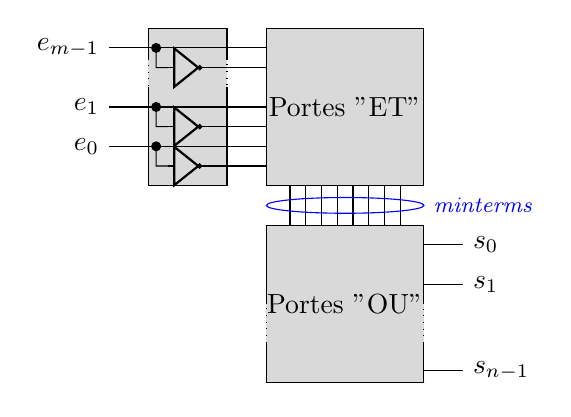
\begin{tikzpicture}
\draw[fill=gray!30, dotted] (0,0) rectangle +(1,2);
\draw (0,1.25) -- (0,0) -- (1,0) -- (1,1.25) (1,1.6) -- (1,2) -- (0,2) -- (0,1.6);
\draw [fill=gray!30] (1.5,0) rectangle +(2,2);
\draw (2.5,1) node[text width=2cm,align=center] {Portes "ET"};

\draw [fill=gray!30,dotted] (1.5,-2.5) rectangle +(2,2);
\draw (1.5,-2) -- ++(0,-.5) -- ++(2,0) -- ++(0,.5) ++ (0,.5) -- ++ (0,1) -- ++(-2,0) -- ++(0,-1);
\draw (2.5,-1.5) node[text width=2cm,align=center] {Portes "OU"};

\draw (-.5,.5) node[left]{$e_0$} -- +(2,0);
\draw (.5,.25) node[not port,scale=.35] (not1) {};
\draw (.1,.5) to[short,*-] ++(0,-.25) -- (not1.in);
\draw (not1.out) -- +(.75,0);

\begin{scope}[yshift=.5cm]
\draw (-.5,.5) node[left]{$e_1$} -- +(2,0);
\draw (.5,.25) node[not port,scale=.35] (not1) {};
\draw (.1,.5) to[short,*-] ++(0,-.25) -- (not1.in);
\draw (not1.out) -- +(.75,0);
\end{scope}

\begin{scope}[yshift=1.25cm]
\draw (-.5,.5) node[left]{$e_{m-1}$} -- +(2,0);
\draw (.5,.25) node[not port,scale=.35] (not1) {};
\draw (.1,.5) to[short,*-] ++(0,-.25) -- (not1.in);
\draw (not1.out) -- +(.75,0);
\end{scope}

\foreach \i in {0,...,7} {
	\draw (1.8 + \i * .2,0) -- +(0,-.5);
	\pgfmathparse{\i < 2}
	\if\pgfmathresult1
	\draw (3.5, -.75 -\i * .5) -- +(.5,0) node[right]{$s_\i$};
	\fi
	\pgfmathparse{\i == 7}
	\if\pgfmathresult1
	\draw (3.5, -.6 -\i * .25) -- +(.5,0) node[right]{$s_{n-1}$};
	\fi
}

\draw[blue] (2.5,-.25) node[right=1cm]{\footnotesize \textit{minterms}} ellipse (1cm and .1cm);

\end{tikzpicture}
\end{center}

\begin{center}
\begin{circuitikz}
\draw (0,0) node[above] {$e_0$} to[short,*-] +(0,-5.5);
\draw (.5,-1) node[not port,rotate=-90,scale=.7] (note0) {};
\draw (0,-.25) to[short,*-]  ++(.5,0) -- (note0.in);
\draw (note0.out) to[short] ++(0,-4.);

\draw (1,0) node[above] {$e_1$} to[short,*-]  +(0,-5.5);
\draw (1.5,-1) node[not port,rotate=-90,scale=.7] (note0) {};
\draw (1,-.25) to[short,*-]  ++(.5,0) -- (note0.in);
\draw (note0.out) to[short] ++(0,-4.);

%% and array

\draw (3,-2) node[and port,scale=.7] (and1) {};
\draw (and1.in 1) to[short,-o,color=blue] ++(-.25,0) to[short,-*] ++(-1.78,0);
\draw (and1.in 1) ++(0,-.13) ++(5pt,0) -- ++(-5pt,0) to[short,-o,color=blue] ++(-.25,0)  to[short,-*] ++(-1.28,0);
\draw (and1.in 2) ++(0,.13) ++(5pt,0) -- ++(-5pt,0) to[short,-o,color=blue] ++(-.25,0) to[short,-*] ++(-0.78,0);
\draw (and1.in 2) to[short,-o,color=blue] ++(-.25,0) to[short,-*] ++(-0.28,0);
\draw (and1.out) -- +(2,0);

\draw (3,-3) node[and port,scale=.7] (and2) {};
\draw (and2.in 1) to[short,-o,color=blue] ++(-.25,0) to[short,-*] ++(-1.78,0);
\draw (and2.in 1) ++(0,-.13) ++(5pt,0) -- ++(-5pt,0) to[short,-o,color=blue] ++(-.25,0)  to[short,-*] ++(-1.28,0);
\draw (and2.in 2) ++(0,.13) ++(5pt,0) -- ++(-5pt,0) to[short,-o,color=blue] ++(-.25,0) to[short,-*] ++(-0.78,0);
\draw (and2.in 2) to[short,-o,color=blue] ++(-.25,0) to[short,-*] ++(-0.28,0);
\draw (and2.out) -- +(2,0);

\draw (3,-4) node[and port,scale=.7] (and3) {};
\draw (and3.in 1) to[short,-o,color=blue] ++(-.25,0) to[short,-*] ++(-1.78,0);
\draw (and3.in 1) ++(0,-.13) ++(5pt,0) -- ++(-5pt,0) to[short,-o,color=blue] ++(-.25,0)  to[short,-*] ++(-1.28,0);
\draw (and3.in 2) ++(0,.13) ++(5pt,0) -- ++(-5pt,0) to[short,-o,color=blue] ++(-.25,0) to[short,-*] ++(-0.78,0);
\draw (and3.in 2) to[short,-o,color=blue] ++(-.25,0) to[short,-*] ++(-0.28,0);
\draw (and3.out) -- +(2,0);

\draw (3,-5) node[and port,scale=.7] (and4) {};
\draw (and4.in 1) to[short,-o,color=blue] ++(-.25,0) to[short,-*] ++(-1.78,0);
\draw (and4.in 1) ++(0,-.13) ++(5pt,0) -- ++(-5pt,0) to[short,-o,color=blue] ++(-.25,0)  to[short,-*] ++(-1.28,0);
\draw (and4.in 2) ++(0,.13) ++(5pt,0) -- ++(-5pt,0) to[short,-o,color=blue] ++(-.25,0) to[short,-*] ++(-0.78,0);
\draw (and4.in 2) to[short,-o,color=blue] ++(-.25,0) to[short,-*] ++(-0.28,0);
\draw (and4.out) -- +(2,0);

%% or array

\draw (3.5,-6.5) node[or port,rotate=-90,scale=.7] (or1) {};
\draw (or1.in 1) to[short,-o,color=blue] ++(0,.25) to[short,-*] ++(0,3.28);
\draw (or1.in 1) ++(-.13,0) ++(0,-9pt) -- ++(0,9pt) to[short,-o,color=blue] ++(0,.25)  to[short,-*] ++(0,2.28);
\draw (or1.in 2) ++(.13,0) ++(0,-9pt) -- ++(0,9pt) to[short,-o,color=blue] ++(0,.25) to[short,-*] ++(0,1.28);
\draw (or1.in 2) to[short,-o,color=blue] ++(0,.25) to[short,-*] ++(0,0.28);
\draw (or1.out) to[short,-*] +(0,-.5) node[below]{$s_0$};

\draw (4.5,-6.5) node[or port,rotate=-90,scale=.7] (or2) {};
\draw (or2.in 1) to[short,-o,color=blue] ++(0,.25) to[short,-*] ++(0,3.28);
\draw (or2.in 1) ++(-.13,0) ++(0,-9pt) -- ++(0,9pt) to[short,-o,color=blue] ++(0,.25)  to[short,-*] ++(0,2.28);
\draw (or2.in 2) ++(.13,0) ++(0,-9pt) -- ++(0,9pt) to[short,-o,color=blue] ++(0,.25) to[short,-*] ++(0,1.28);
\draw (or2.in 2) to[short,-o,color=blue] ++(0,.25) to[short,-*] ++(0,0.28);
\draw (or2.out) to[short,-*] +(0,-.5) node[below]{$s_1$};
\end{circuitikz}
\end{center}

\begin{center}
\begin{circuitikz}
\draw (0,0) node[above] {$a$} to[short,*-] +(0,-5.5);
\draw (.5,-1) node[not port,rotate=-90,scale=.7] (note0) {};
\draw (0,-.25) to[short,*-]  ++(.5,0) -- (note0.in);
\draw (note0.out) to[short] ++(0,-4.);

\draw (1,0) node[above] {$b$} to[short,*-]  +(0,-5.5);
\draw (1.5,-1) node[not port,rotate=-90,scale=.7] (note0) {};
\draw (1,-.25) to[short,*-]  ++(.5,0) -- (note0.in);
\draw (note0.out) to[short] ++(0,-4.);

%% and array

\draw (3,-2) node[and port,scale=.7] (and1) {};
\draw (and1.in 1) to[short,-o,color=blue] ++(-.25,0) to[short,-*] ++(-1.78,0);
\draw (and1.in 1) ++(0,-.13) ++(5pt,0) -- ++(-5pt,0)  ++(-.25,0)  to[short,-*] ++(-1.28,0);
\draw (and1.in 2) ++(0,.13) ++(5pt,0) -- ++(-5pt,0)to[short,-o,color=blue] ++(-.25,0) to[short,-*] ++(-0.78,0);
\draw (and1.in 2)  ++(-.25,0) to[short,-*] ++(-0.28,0);
\draw (and1.out) -- +(2,0);

\draw (3,-3) node[and port,scale=.7] (and2) {};
\draw (and2.in 1) ++(-.25,0) to[short,-*] ++(-1.78,0);
\draw (and2.in 1) ++(0,-.13) ++(5pt,0) -- ++(-5pt,0) to[short,-o,color=blue] ++(-.25,0)  to[short,-*] ++(-1.28,0);
\draw (and2.in 2) ++(0,.13) ++(5pt,0) -- ++(-5pt,0) to[short,-o,color=blue] ++(-.25,0) to[short,-*] ++(-0.78,0);
\draw (and2.in 2)  ++(-.25,0) to[short,-*] ++(-0.28,0);
\draw (and2.out) -- +(2,0);

\draw (3,-4) node[and port,scale=.7] (and3) {};
\draw (and3.in 1) ++(-.25,0) to[short,-*] ++(-1.78,0);
\draw (and3.in 1) ++(0,-.13) ++(5pt,0) -- ++(-5pt,0) to[short,-o,color=blue] ++(-.25,0)  to[short,-*] ++(-1.28,0);
\draw (and3.in 2) ++(0,.13) ++(5pt,0) -- ++(-5pt,0)  ++(-.25,0) to[short,-*] ++(-0.78,0);
\draw (and3.in 2) to[short,-o,color=blue] ++(-.25,0) to[short,-*] ++(-0.28,0);
\draw (and3.out) -- +(2,0);

\draw (3,-5) node[and port,scale=.7] (and4) {};
\draw (and4.in 1) to[short,-o,color=blue] ++(-.25,0) to[short,-*] ++(-1.78,0);
\draw (and4.in 1) ++(0,-.13) ++(5pt,0) -- ++(-5pt,0)  ++(-.25,0)  to[short,-*] ++(-1.28,0);
\draw (and4.in 2) ++(0,.13) ++(5pt,0) -- ++(-5pt,0)  ++(-.25,0) to[short,-*] ++(-0.78,0);
\draw (and4.in 2) to[short,-o,color=blue] ++(-.25,0) to[short,-*] ++(-0.28,0);
\draw (and4.out) -- +(2,0);

%% or array

\draw (3.5,-6.5) node[or port,rotate=-90,scale=.7] (or1) {};
\draw (or1.in 1) to[short,-o,color=blue] ++(0,.25) to[short,-*] ++(0,3.28);
\draw (or1.in 1) ++(-.13,0) ++(0,-9pt) -- ++(0,9pt) to[short,-o,color=blue] ++(0,.25)  to[short,-*] ++(0,2.28);
\draw (or1.in 2) ++(.13,0) ++(0,-9pt) -- ++(0,9pt)  ++(0,.25) to[short,-*] ++(0,1.28);
\draw (or1.in 2)  ++(0,.25) to[short,-*] ++(0,0.28);
\draw (or1.out) to[short,-*] +(0,-.5) node[below]{$f$};

\draw (4.5,-6.5) node[or port,rotate=-90,scale=.7] (or2) {};
\draw (or2.in 1)  ++(0,.25) to[short,-*] ++(0,3.28);
\draw (or2.in 1) ++(-.13,0) ++(0,-9pt) -- ++(0,9pt)  ++(0,.25)  to[short,-*] ++(0,2.28);
\draw (or2.in 2) ++(.13,0) ++(0,-9pt) -- ++(0,9pt) to[short,-o,color=blue] ++(0,.25) to[short,-*] ++(0,1.28);
\draw (or2.in 2) to[short,-o,color=blue] ++(0,.25) to[short,-*] ++(0,0.28);
\draw (or2.out) to[short,-*] +(0,-.5) node[below]{$g$};
\end{circuitikz}
\end{center}

\begin{center}

\newcommand{\andxx}[1]{
\draw[thick] (#1) .. controls +(0,.25) and +(.25,0) .. ++(-.8,.4)  -- ++(0,-.8) .. controls +(.25,0) and +(0,-.25) .. cycle;
}

\newcommand{\orxx}[1]{
% .. controls +(0,.25) and +(.25,0) ..
\draw[thick] (#1) .. controls +(-.25,0) and +(0,-.25) ..  ++(-.4,.8)  .. controls +(-45:.3) and +(-45-90:.3) .. ++(.8,0) .. controls +(0,-.25) and +(.25,0) .. cycle;
}

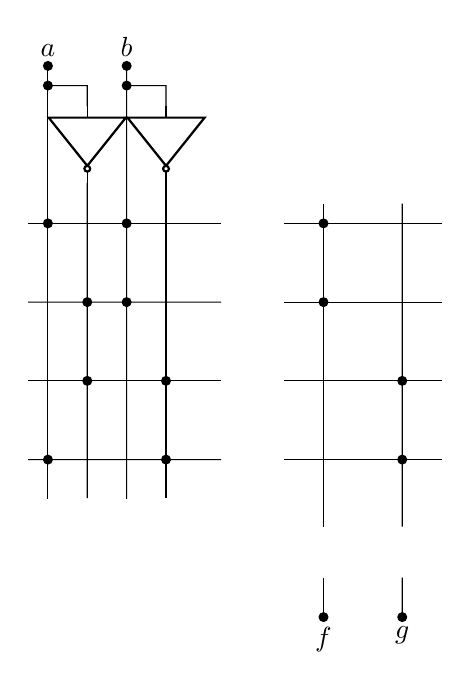
\begin{tikzpicture}
\draw (0,0) node[above] {$a$} to[short,*-] +(0,-5.5);
\draw (.5,-1) node[not port,rotate=-90,scale=.7] (note0) {};
\draw (0,-.25) to[short,*-]  ++(.5,0) -- (note0.in);
\draw (note0.out) to[short] ++(0,-4.);

\draw (1,0) node[above] {$b$} to[short,*-]  +(0,-5.5);
\draw (1.5,-1) node[not port,rotate=-90,scale=.7] (note0) {};
\draw (1,-.25) to[short,*-]  ++(.5,0) -- (note0.in);
\draw (note0.out) to[short] ++(0,-4.);

%% and array
\node (and1) at (3,-2) {};
\andxx{and1.center}
\draw (and1) ++(-.8,0) -- ++(-.2,0) to [short,-*] ++(-1,0) to [short,-*] ++(-1,0) -- ++(-.25,0);
\draw (and1.center) -- +(2,0);

\node (and2) at (3,-3) {};
\andxx{and2.center}
\draw (and2) ++(-.8,0) -- ++(-.2,0) to [short,-*] ++(-1,0) to [short,-*] ++(-.5,0) -- ++(-.5,0)-- ++(-.25,0);
\draw (and2.center) -- +(2,0);


\node (and3) at (3,-4) {};
\andxx{and3.center}
\draw (and3) ++(-.8,0) -- ++(-.2,0) to [short,-*] ++(-.5,0) to [short,-*] ++(-1,0) -- ++(-.5,0)-- ++(-.25,0);
\draw (and3.center) -- +(2,0);

\node (and4) at (3,-5) {};
\andxx{and4.center}
\draw (and4) ++(-.8,0) -- ++(-.2,0) to [short,-*] ++(-.5,0) to [short,-*] ++(-1.5,0)-- ++(-.25,0);
\draw (and4.center) -- +(2,0);

%% or array

\node (or1) at (3.5,-6.5) {};
\orxx{or1.center}
\draw (or1) ++(0,.65) -- ++(0,.35) to [short,-*] ++(0,2.5) to [short,-*] ++(0,1)-- ++(0,.25);
\draw (or1.center) to[short,-*] +(0,-.5) node[below]{$f$};

\node (or1) at (4.5,-6.5) {};
\orxx{or1.center}
\draw (or1) ++(0,.65) -- ++(0,.35) to [short,-*] ++(0,0.5) to [short,-*] ++(0,1)-- ++(0,2.25);
\draw (or1.center) to[short,-*] +(0,-.5) node[below]{$g$};
\end{tikzpicture}
\end{center}

\begin{center}
\begin{circuitikz}
\draw (0,0) node[or port] (orx) {};
\draw (orx.in 1) to[short,-*] +(-.5,0) node[left] {$a$};
\draw (orx.out) to[short,-*] ++(1.5,0) node[right] {$r(a)$};
\draw (orx.out) ++(.5,0) to[short,*-] ++ (0,-1) to[short] ++(-2.04,0) to [short] (orx.in 2);
\end{circuitikz}
\end{center}

\makeatletter
\newcommand{\gettikzxy}[3]{%
  \tikz@scan@one@point\pgfutil@firstofone#1\relax
  \edef#2{\the\pgf@x}%
  \edef#3{\the\pgf@y}%
}
\makeatother

\begin{center}
\begin{circuitikz}
\draw (0,2) node[nor port] (or2) {};
\draw (or2.in 1) to[short,-*] +(-.5,0) node[left] {$S$};
\draw (or2.out) to[short,-*] ++(1.5,0) node[right] {$\bar Q$};
\draw (0,0) node[nor port] (or1) {};
\draw (or1.in 2) to[short,-*] +(-.5,0) node[left] {$R$};
\draw (or1.out) to[short,-*] ++(1.5,0) node[right] {$Q$};

\gettikzxy{(or2.in 2)}{\ax}{\ay}
\draw (or1.out) ++(.5,0) to[short,*-] (\ax - .25 cm, \ay) to[short] +(.25,0);
\gettikzxy{(or1.in 1)}{\ax}{\ay}
\draw (or2.out) ++(.5,0) to[short,*-] (\ax - .25 cm, \ay) to[short] +(.25,0);
\end{circuitikz}
\end{center}

\begin{center}
\begin{circuitikz}
\draw (0,3) node[and port] (and2) {};
\draw (and2.in 1) to[short,-*] +(-.5,0) node[left] {$S$};

\draw (0,0) node [and port] (and1) {};
\draw (and1.in 2) to[short,-*] +(-.5,0) node[left] {$R$};

\draw (and2.in 2) to[short] (and1.in 1);
\gettikzxy{(and2.in 2)}{\ax}{\ay}
\draw (\ax, 1.5) to[short,*-*] +(-.5,0) node[left]{$E$};


\gettikzxy{(and2.in 2)}{\ax}{\ay}
\draw (\ax + 2.9 cm, \ay) node[nor port] (or2) {};
\draw (or2.out) to[short,-*] ++(1.5,0) node[right] {$\bar Q$};

\gettikzxy{(and1.in 1)}{\ax}{\ay}
\draw (\ax + 2.9 cm, \ay) node[nor port] (or1) {};
\draw (or1.out) to[short,-*] ++(1.5,0) node[right] {$Q$};

\gettikzxy{(or2.in 2)}{\ax}{\ay}
\draw (or1.out) ++(.5,0) to[short,*-] (\ax - .25 cm, \ay) to[short] +(.25,0);
\gettikzxy{(or1.in 1)}{\ax}{\ay}
\draw (or2.out) ++(.5,0) to[short,*-] (\ax - .25 cm, \ay) to[short] +(.25,0);
\end{circuitikz}
\end{center}

\begin{center}
\begin{circuitikz}
\draw (0,3) node[and port] (and2) {};
\draw (and2.in 1) to[short,-*] +(-2,0) node[left] {$D$};

\draw (0,0) node [and port] (and1) {};

\draw (and2.in 1) ++(-.75,-2.75) node[not port,rotate=-90] (notx) {};

\gettikzxy{(and2.in 1)}{\ax}{\ay};
\draw(notx.in) to[short,-*] (\ax-.75 cm,\ay);
\gettikzxy{(and1.in 2)}{\ax}{\ay};
\draw (notx.out) to[short] (\ax-.75 cm,\ay) to[short] (\ax,\ay);

\draw (and2.in 2) to[short] (and1.in 1);
\gettikzxy{(and2.in 2)}{\ax}{\ay}
\draw (\ax, 1.5) to[short,*-*] +(-2,0) node[left]{$E$};


\gettikzxy{(and2.in 2)}{\ax}{\ay}
\draw (\ax + 2.9 cm, \ay) node[nor port] (or2) {};
\draw (or2.out) to[short,-*] ++(1.5,0) node[right] {$\bar Q$};

\gettikzxy{(and1.in 1)}{\ax}{\ay}
\draw (\ax + 2.9 cm, \ay) node[nor port] (or1) {};
\draw (or1.out) to[short,-*] ++(1.5,0) node[right] {$Q$};

\gettikzxy{(or2.in 2)}{\ax}{\ay}
\draw (or1.out) ++(.5,0) to[short,*-] (\ax - .25 cm, \ay) to[short] +(.25,0);
\gettikzxy{(or1.in 1)}{\ax}{\ay}
\draw (or2.out) ++(.5,0) to[short,*-] (\ax - .25 cm, \ay) to[short] +(.25,0);
\end{circuitikz}
\end{center}

\begin{center}
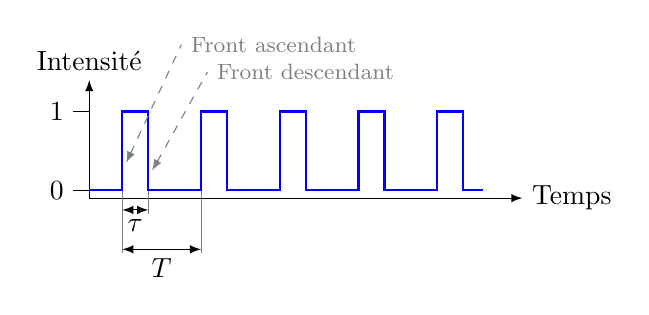
\begin{tikzpicture}
\draw[-latex] (-.75,0-.1) -- +(5.5,0) node[right]{Temps};
\draw[-latex] (-.75,0-.1) -- +(0,1.5) node[above]{Intensité};
\draw (-.75,0) -- +(-.2,0) node[left]{0};
\draw (-.75,1) -- +(-.2,0) node[left]{1};

\edef\taux{.33}
\draw[gray] (-\taux,0) -- +(0,-.8);
\draw[gray] (0,0) -- +(0,-.3);
\draw[gray] (-\taux + 1,0) -- +(0,-.8);
\foreach \i in {0,...,4} {
	\draw[blue,thick] (\i-.75,0) -- (\i -\taux,0) -- (\i - \taux, 1) -- (\i, 1) -- (\i,0) -- (\i + .25, 0);
}
\draw [gray,latex-,dashed] (0-\taux+.05,.35) -- +(.7,1.5) node[right]{\footnotesize Front ascendant};
\draw [gray,latex-,dashed] (0.05,.25) -- +(.7,1.25) node[right]{\footnotesize Front descendant};
\draw[latex-latex] (-\taux,-.25) -- node[midway,below]{$\tau$} +(\taux,0); 
\draw[latex-latex] (-\taux,-.75) -- node[midway,below]{$T$} +(1,0); 
\end{tikzpicture}
\end{center}

\begin{center}

\begin{circuitikz}
\def\lll{2.5}
\draw (\lll,0) node[and port] (andx) {};
\draw (andx.in 1) -- +(-\lll,0) node[left]{$a$} ;
\draw (andx.out) to[short,-*] +(.5,0) node[right]{$\bar a \cdot a$} ;
\draw (\lll-2.5,-.75) node[not port] (nots) {};
\draw (nots.in) to[short,-*] ++(0,1.03);
\gettikzxy{(andx.in 2)}{\ax}{\ay}
\gettikzxy{(nots.out)}{\bx}{\by}
\draw (nots.out) node[below,blue]{$\overline{a}$} -- (\bx,\ay) -- (\ax,\ay) ;
\end{circuitikz}

\vspace{.5cm}
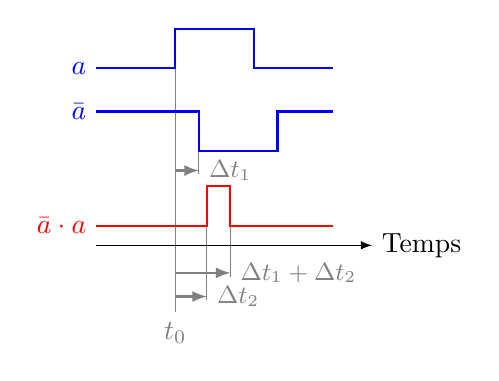
\begin{tikzpicture}
\draw[gray] (1,0) -- +(0,-3.1) node[below]{$t_0$};
\draw[blue,thick] (0,0) node[left]{$a$} -- ++(1,0) -- ++(0,.5) -- ++(1,0) -- ++(0,-.5) -- ++(1,0);
\draw[gray] (1.3,-.75) -- +(0,-.6);
\draw[blue,thick] (0,-.55) node[left]{$\bar a$} -- ++(1+.3,0) -- ++(0,-.5) -- ++(1,0) -- ++(0,.5) -- ++(.7,0);
\draw [gray,-latex,thick] (1,-1.3) -- +(.3,0) node[right]{\small $\Delta{t}_1$};
\draw[gray] (1.4,-2) -- +(0,-.95);
\draw[gray] (1.7,-2) -- +(0,-.65);
\draw[red,thick] (0,-2) node[left]{$\bar a \cdot a$} -- ++(1+.4,0) -- ++(0,.5) -- ++(.3,0) -- ++(0,-.5) -- ++(1.3,0);
\draw [gray,-latex,thick] (1,-2.6) -- +(.7,0) node[right]{\small $\Delta{t}_1+\Delta{t}_2$};
\draw [gray,-latex,thick] (1,-2.9) -- +(.4,0) node[right]{\small $\Delta{t}_2$};
\draw[-latex](0,-2.25) -- +(3.5,0) node[right]{Temps};
\end{tikzpicture}

\end{center}

\begin{center}
\begin{circuitikz}

\draw[fill=yellow!10] (-3,4) rectangle (2.75,-1);
\draw (0,3) node[and port] (and2) {};
\draw (and2.in 1) to[short,-*] +(-2,0) node[left] {$D$};

\draw (0,0) node [and port] (and1) {};

\draw (and2.in 1) ++(-.75,-2.75) node[not port,rotate=-90] (notx) {};

\gettikzxy{(and2.in 1)}{\ax}{\ay};
\draw(notx.in) to[short,-*] (\ax-.75 cm,\ay);
\gettikzxy{(and1.in 2)}{\ax}{\ay};
\draw (notx.out) to[short] (\ax-.75 cm,\ay) to[short] (\ax,\ay);

\draw (and2.in 2) to[short] (and1.in 1);
\gettikzxy{(and1.in 1)}{\ax}{\ay}
\draw (\ax, \ay) to[short,*-] ++(0,-2)  to[short,-*] ++(-2,0) node[left]{$C$};


\gettikzxy{(and2.in 2)}{\ax}{\ay}
\draw (\ax + 2.9 cm, \ay) node[nor port] (or2) {};
\draw (or2.out) to[short] ++(.5,0);

\gettikzxy{(and1.in 1)}{\ax}{\ay}
\draw (\ax + 2.9 cm, \ay) node[nor port] (or1) {};
\draw (or1.out) to[short] ++(2,0);

\gettikzxy{(or2.in 2)}{\ax}{\ay}
\draw (or1.out) ++(.5,0) to[short,*-] (\ax - .25 cm, \ay) to[short] +(.25,0);
\gettikzxy{(or1.in 1)}{\ax}{\ay}
\draw (or2.out) ++(.5,0) to[short] (\ax - .25 cm, \ay) to[short] +(.25,0);

\begin{scope}[xshift=6cm,yshift=-3cm]
\draw[fill=yellow!10] (-3,4) rectangle (2.75,-1);
\draw (0,3) node[and port] (and2) {};
\draw (and2.in 1) to[short] +(-2,0);

\draw (0,0) node [and port] (and1) {};

\draw (and2.in 1) ++(-.75,-2.75) node[not port,rotate=-90] (notx) {};

\gettikzxy{(and2.in 1)}{\ax}{\ay};
\draw(notx.in) to[short,-*] (\ax-.75 cm,\ay);
\gettikzxy{(and1.in 2)}{\ax}{\ay};
\draw (notx.out) to[short] (\ax-.75 cm,\ay) to[short] (\ax,\ay);

\draw (and2.in 2) to[short] (and1.in 1);
\gettikzxy{(and2.in 2)}{\ax}{\ay}
\draw (\ax,\ay) ++(-3,-1.44)  node[not port] (notc) {};
\draw (\ax, \ay) ++(0,-1.44) to[short,*-] (notc.out) (notc.in) to[short,-*] ++(-2.295,0);


\gettikzxy{(and2.in 2)}{\ax}{\ay}
\draw (\ax + 2.9 cm, \ay) node[nor port] (or2) {};
\draw (or2.out) to[short,-*] ++(1.5,0) node[right] {$\bar Q$};

\gettikzxy{(and1.in 1)}{\ax}{\ay}
\draw (\ax + 2.9 cm, \ay) node[nor port] (or1) {};
\draw (or1.out) to[short,-*] ++(1.5,0) node[right] {$Q$};

\gettikzxy{(or2.in 2)}{\ax}{\ay}
\draw (or1.out) ++(.5,0) to[short,*-] (\ax - .25 cm, \ay) to[short] +(.25,0);
\gettikzxy{(or1.in 1)}{\ax}{\ay}
\draw (or2.out) ++(.5,0) to[short,*-] (\ax - .25 cm, \ay) to[short] +(.25,0);
\end{scope}
\end{circuitikz}
\end{center}


\begin{center}
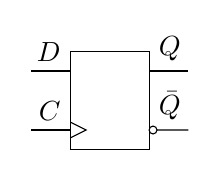
\begin{tikzpicture}
\draw (0,0) rectangle +(1,1.25);
\draw (0,1.) node[anchor=south east]{$D$}-- +(-.5,0); 
\draw (0,.25) node[anchor=south east]{$C$}-- +(-.5,0); 
\draw (0,.25) ++(0,.1) -- ++ (.2,-.1) -- ++(-.2,-.1);
\draw (1,1.) node[anchor=south west]{$Q$}-- +(.5,0); 
\draw (1,.25) node[anchor=south west]{$\bar Q$} ++(.05,0) circle (.05cm) ++(.05,0)  -- +(.4,0); 
\end{tikzpicture}
\hspace{1cm}
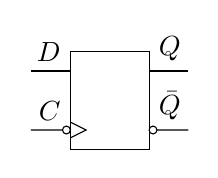
\begin{tikzpicture}
\draw (0,0) rectangle +(1,1.25);
\draw (0,1.) node[anchor=south east]{$D$}-- +(-.5,0); 
\draw (0,.25) node[anchor=south east]{$C$}++(-.05,0) circle (.05cm) ++(-.05,0)  -- +(-.4,0); 
\draw (0,.25) ++(0,.1) -- ++ (.2,-.1) -- ++(-.2,-.1);
\draw (1,1.) node[anchor=south west]{$Q$}-- +(.5,0); 
\draw (1,.25) node[anchor=south west]{$\bar Q$} ++(.05,0) circle (.05cm) ++(.05,0)  -- +(.4,0); 
\end{tikzpicture}

\end{center}

\begin{center}
\begin{circuitikz}

\draw[fill=gray!20] (-3.25,1.5) rectangle +(12,-2.75);

\draw (-1,-.5) node[and port] (and1) {};
\draw (and1.out) -- ++(5,0) ++(1,0) -- ++(1.4,0);
\draw[dotted] (and1.out)  ++(5,0) -- ++(1,0);
\draw[latex-] (and1.in 2) -- ++(-1,0) node[left]{$w$};
\draw[latex-] (and1.in 1) -- ++(-.5,0) -- ++(0,2) node[above]{$C$};
\begin{scope}
\draw (0,0) rectangle +(1,1.25);
\draw[latex-] (0,1.) -- ++(-.5,0) -- ++(0,.75) node[above]{$d_0$}; 
\draw (0,.25) -- ++(-.5,0) to[short,-*] ++(0,-.75); 
\draw (0,.25) ++(0,.1) -- ++ (.2,-.1) -- ++(-.2,-.1);
\draw[-latex] (1,1.) -- ++(.5,0) -- ++(0,.75) node[above]{$a_0$}; 
\draw (1,.25) ++(.05,0) circle (.05cm) ++(.05,0)  -- +(.4,0); 
\end{scope}
\begin{scope}[xshift=3cm]
\draw (0,0) rectangle +(1,1.25);
\draw[latex-] (0,1.) -- ++(-.5,0) -- ++(0,.75) node[above]{$d_1$}; 
\draw (0,.25) -- ++(-.5,0) to[short,-*] ++(0,-.75); 
\draw (0,.25) ++(0,.1) -- ++ (.2,-.1) -- ++(-.2,-.1);
\draw[-latex] (1,1.) -- ++(.5,0) -- ++(0,.75) node[above]{$a_1$}; 
\draw (1,.25) ++(.05,0) circle (.05cm) ++(.05,0)  -- +(.4,0); 
\end{scope}

\begin{scope}[xshift=7cm]
\draw (0,0) rectangle +(1,1.25);
\draw[latex-] (0,1.) -- ++(-.5,0) -- ++(0,.75) node[above]{$d_{n-1}$}; 
\draw (0,.25) -- ++(-.5,0) to[short,-*] ++(0,-.75); 
\draw (0,.25) ++(0,.1) -- ++ (.2,-.1) -- ++(-.2,-.1);
\draw[-latex] (1,1.) -- ++(.5,0) -- ++(0,.75) node[above]{$a_{n-1}$}; 
\draw (1,.25) ++(.05,0) circle (.05cm) ++(.05,0)  -- +(.4,0); 
\end{scope}
\end{circuitikz}
\end{center}

\begin{center}
\begin{circuitikz}
\draw[red] (-1.5,1.49) -- +(2.5,0) node[right]{\textit{word line}};
\draw[blue] (-1,2) -- +(0,-2.5) node[below]{\textit{bit line}};
\draw (0,0) node[nmos, rotate=-90] (nmos1) {};
\draw (nmos1.E) to[short,-*] (-1,0);
\draw (nmos1.C) to[short] (1,0) to[C] ++(0,-1) node[ground] {};
\draw (nmos1.B) to[short,-*] +(0,.5);
\end{circuitikz}
\end{center}

\end{document}